\documentclass[a4paper]{report}
% Shared preamble for the English probability and statistics documents.
% Based on the original course preamble. Compile with pdfLaTeX.
\usepackage[top=1.5cm,bottom=2cm,left=2cm,right=2cm]{geometry}
\usepackage[T1]{fontenc}
\usepackage{lmodern}
\usepackage[utf8]{inputenc}
\usepackage[english]{babel}

\usepackage{amsmath}
\usepackage{amssymb}
\usepackage{amsthm}
\usepackage{mathrsfs}
\usepackage{mathtools}
\usepackage{etoolbox}
\usepackage{tikz}
\usetikzlibrary{shapes.multipart,arrows.meta}
\usepackage{xcolor}
\usepackage{enumerate}
\usepackage[shortlabels]{enumitem}
\usepackage{hyperref}
\usepackage{version}
\usepackage{bbold}
\usepackage{fontawesome5}
\usepackage{fancyhdr}
\lfoot{}
\usepackage{natbib}
\usepackage{graphicx}
\usepackage{pdfpages}
\usepackage{authblk}
    
\usepackage{blindtext}
\usepackage{multicol}
\usepackage{collcell}
\usepackage{wrapfig}
\usepackage{blkarray}
\usepackage{cancel}
\usepackage{appendix}
\usepackage{float}
\makeatletter
\input{tex/assets/slashbox.sty}
\makeatother
\hypersetup{unicode,colorlinks,citecolor=red,filecolor=black,
  linkcolor=red,urlcolor=cyan}
\setlength{\columnsep}{1cm}
\pagenumbering{gobble}

\def\numtext#1{%
  \ifcase#1\or one\or two\or three\or four\or five\or six\or seven\or eight\or nine\or ten\or
  eleven\or twelve\or thirteen\or fourteen\or fifteen\or sixteen\or seventeen\or eighteen\or nineteen\or twenty\or Lots\fi}

\newcommand{\Byte}[1]{%
  \def\nodecontents{}%
  \foreach[count=\l] \k in {#1} {\xappto{\nodecontents}{\noexpand\nodepart{\numtext{\l}}\k}}%
  \node[rectangle split,rectangle split parts=8,rectangle split horizontal,draw] at (2,2){\nodecontents};}

\newcommand{\D}{{\mathrm{d}}}
\newcommand{\cE}{{\mathcal{E}}}
\newcommand{\cG}{{\mathcal{G}}}
\newcommand{\cX}{{\mathcal{X}}}
\newcommand{\cY}{{\mathcal{Y}}}
\newcommand{\cB}{{\mathcal{B}}}
\newcommand{\cF}{{\mathcal{F}}}
\newcommand{\cO}{{\mathcal{O}}}
\newcommand{\cS}{{\mathcal{S}}}
\newcommand{\cT}{{\mathcal{T}}}
\newcommand{\given}{\, \big| \,}
\newcommand{\cL}{{\mathscr{L}}}
\newcommand{\cD}{{\mathcal{D}}}
\newcommand{\cA}{{\mathscr{A}}}
\newcommand{\cP}{{\mathscr{P}}}
\newcommand{\cR}{{\mathscr{R}}}
\newcommand{\A}{{\mathcal A}}
\newcommand{\one}{\mathbb{1}}
\newcommand{\mathbbm}[1]{\mathbb{#1}}

\providecommand{\C}{}
\renewcommand{\C}{\mathbb C}
\newcommand{\R}{\mathbb R}
\newcommand{\Q}{\mathbb Q}
\newcommand{\N}{\mathbb N}
\newcommand{\T}{\mathbb T}
\newcommand{\F}{\mathbb F}
\renewcommand{\P}{\mathbb P}
\newcommand{\Z}{\mathbb Z}
\newcommand{\E}{\mathbb {E}}
\newcommand{\Pbb}[1]{\P\left( #1\right)}
\newcommand{\Ebb}[1]{\E\left[ #1\right]}

\newcommand{\lb}{\left (}
\newcommand{\rb}{\right )}
\newcommand{\lbb}{\left [}
\newcommand{\rbb}{\right ]}
\newcommand{\labs}{\left |}
\newcommand{\rabs}{\right |}
\newcommand{\lbrb}[1]{\lb #1 \rb}
\newcommand{\lbbrbb}[1]{\lbb#1\rbb}
\newcommand{\labsrabs}[1]{\labs#1\rabs}
\newcommand{\lbbrb}[1]{\lbb#1\rb}
\newcommand{\lbrbb}[1]{\lb#1\rbb}
\newcommand{\langlerangle}[1]{\langle#1\rangle}
\newcommand{\lbcurly}{\{}
\newcommand{\rbcurly}{\}}
\newcommand{\curly}[1]{\lbcurly#1\rbcurly}
\newcommand{\abs}{\labsrabs}
\newcommand{\ind}[1]{1_{#1}}
\newcommand{\indep}{\perp \!\!\! \perp}
\renewcommand{\d}{\, \mathrm{d}}

\newtheorem{theorem}{Theorem}
\newtheorem{problemCnt}{Lemma}
\theoremstyle{definition}
\newtheorem{problem}[problemCnt]{Problem}
\newtheorem{problembook}[problemCnt]{\faBook \,  Problem}
\newtheorem{problempencil}[problemCnt]{\faPencil* \,  Problem}
\newtheorem{problemstar}[problemCnt]{\faStar\,  Problem}
\newtheorem{problemstarpencil}[problemCnt]{\faStar \, \faPencil* \,   Problem}
\newtheorem{probleminteresting}[problemCnt]{\faSmile[regular] \,   Problem}
\newtheorem{solution}{Solution}

\newcommand{\fwcell}[1]{\makebox[\arraystretch\normalbaselineskip]{$#1$}}
\newenvironment{enumeratei}{\begin{enumerate}[(i)]}{\end{enumerate}}
\newenvironment{enumeratea}{\begin{enumerate}[(a)]}{\end{enumerate}}
\newenvironment{enumeraten}{\begin{enumerate}[\upshape 1.]}{\end{enumerate}}

% Compatibility helpers needed by a few files in the combined archive.
\AtBeginDocument{\noindent{\footnotesize English translation prepared with ChatGPT (OpenAI, GPT-6), 26 October 2026, for translation of the Bulgarian text into English and LaTeX formatting.
The Bulgarian originals remain the reference; translation may contain errors.}\par\smallskip}
\newcommand{\MissingGraphic}[1]{%
  \begin{center}\fbox{\parbox{0.82\linewidth}{\centering Missing source image: \texttt{#1}}}\end{center}}



\begin{document}
\noindent Probability and Statistics, CS Year 3, 2021/2022 \hfill Test 1
\hrulefill
\begin{it}Your grade is 2 + the number of points. Time allowed: 150 minutes. Good luck! Work on $(\Omega,\mathcal F,\P)$. Unless otherwise stated, a random choice is uniform.\end{it}
\begin{problem} (1 point)
One box contains an ordinary six-sided die, another a fair eight-sided die labelled 1 through 8. Ivan chooses a box at random, rolls its die and announces the result. As a function of the announced number, what is the probability that it came from the ordinary die?
\end{problem}
\begin{problem} (1 point)
Approximate the numbers of first-, second- and third-year students by 600, 400 and 200, respectively. Their probabilities of attending a class are 80\%, 60\% and 25\%. Choose two random students who attended classes. Given that they are from different years, what is the probability the more senior is in year 3?
\end{problem}
\begin{problem}
An examination has 20 questions, each with four possible answers. A student knows ten answers and answers them correctly, and guesses the other ten at random. Let $X$ count correct answers. Find:
\begin{enumerate}
\item (0.3 points) the distribution of $X$;
\item (0.3 points) $\P(X>15)$;
\item (0.4 points) $\E X$ and $DX$. Full credit requires explicit answers; calculations can avoid binomial coefficients.
\end{enumerate}
\end{problem}
\begin{problem}
A message consists of eight bits. Noise between servers causes each bit to be transmitted incorrectly with probability $p$.
\begin{center}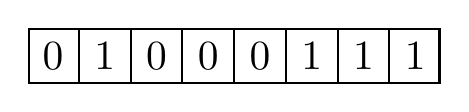
\begin{tikzpicture}[thick,scale=0.6,every node/.style={scale=1.5}]\Byte{0,1,0,0,0,1,1,1}\end{tikzpicture}\end{center}
\begin{enumerate}
\item (0.5 points) What is the probability that a message is transmitted correctly between directly connected servers $A,B$? What is the expected number of correct bits in the final message?
\item (0.5 points) Answer the same questions if the message passes exactly once through each of $n=3$ intermediate servers. Bonus: what happens as $n\to\infty$?
\end{enumerate}
\end{problem}
\end{document}
